\chapter{Relaciones para el ajuste de una elipse}
% \markboth{}{Appendix A}
\label{app:ellipse_formulae}

Para obtener las incertezas estad\'isticas en los \acp{FF} de shift y stretch se utiliza un ajuste a una elipse, siguiendo los pasos sugeridos en la \Refn{\cite{FitEllipse}}. Como salida del ajuste se obtienen un conjunto de par\'ametros \(\{A,B,C,D,E,F\}\) que parametriza la c\'onica:
\begin{equation*}
    F(x,y) = Ax^2 + Bxy + Cy^2 + Dx + Ey + F = 0,
\end{equation*}
con \(B^2 - 4AC < 0\) para el caso de elipses.
Las variables \(x,y\) mostradas son generales, pero en el caso de \acp{FF}, representan los par\'ametros de shift y stretch, respectivamente. Este set de par\'ametros es transformado para obtener la forma can\'onica de una elipse:
\begin{equation*}
    \frac{((x-x_0)\cos\theta + (y-y_0)\sin\theta)^2}{a^2} + \frac{((x-x_0)\sin\theta - (y-y_0)\cos\theta)^2}{b^2} = 1,
\end{equation*}
de donde se puede extraer el centro de la elipse dado por \((x_0, y_0)\), su \'angulo de inclinaci\'on \(\theta\) y los semiejes mayor y menor, \(a\) and \(b\), respectivamente. Luego, las incertezas deseadas en \(x\) e \(y\), junto con su correlaci\'on se puede obtener mediante las relaciones (ver \Fig{\ref{fig:ellipse_formulae:ellipse}}):
\begin{gather}
    \sigma_x = \sqrt{a^2 \cos^2\theta + b^2 \sin^2\theta}\\
    \sigma_y = \sqrt{a^2 \sin^2\theta + b^2 \cos^2\theta}\\
    \rho = \tan(2\theta) \frac{\sigma_{x}^2-\sigma_{y}^2}{2\sigma_{x}\sigma_{y}}.
\end{gather}

\begin{figure}[ht!]
    \centering
    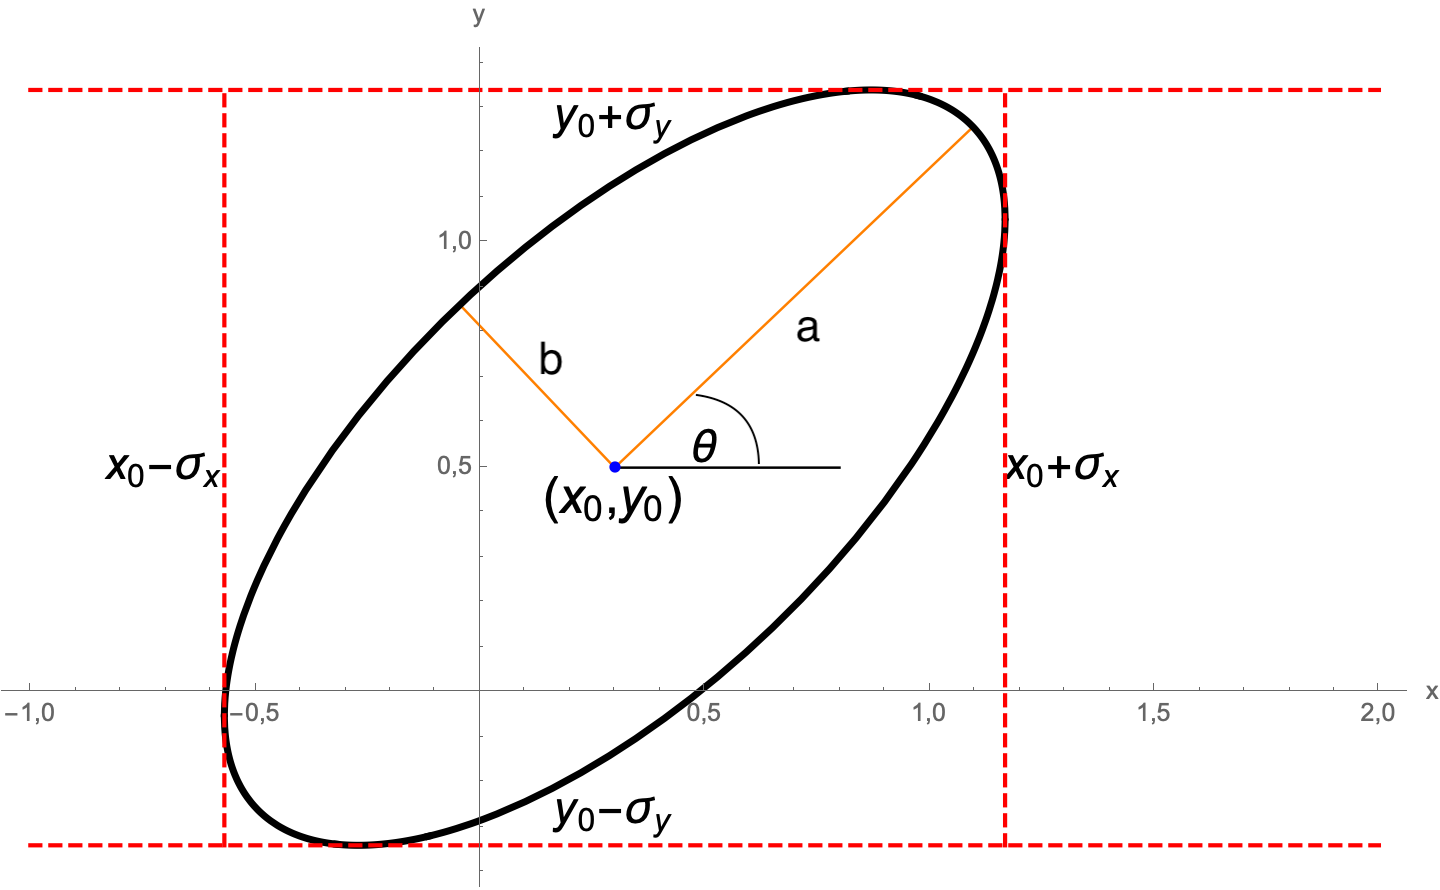
\includegraphics[width=0.5\linewidth]{4_photonid/ffs/procedure/ellipse}
    \caption{Par\'ameteros de una elipse.}
    \label{fig:ellipse_formulae:ellipse}
\end{figure}
